\section{Electromagnetism}
\subsection{Concept of a magnetic field}
\textbf{Magnets} produce magnetic fields. 
\begin{itemize}
\item Hard magnetic materials like cobalt and nickel are difficult to magnetise but tend to retain their magnetism.
\item Soft magnetic materials like iron are easily magnetised but tend to lose their magnetism easily.
\end{itemize}

\begin{defn}{Magnetic field}{}
Region of space where a magnetic pole, a current-carrying conductor or a moving charge particle will experience a force.
\end{defn}

A magnetic field can be produced by:
\begin{enumerate}
\item permanent magnets
\item current-carrying conductors
\end{enumerate}

\subsubsection{Magnetic field lines}
\begin{itemize}
\item The field is represented by lines of force, starting from the North pole and ending at the South pole.
\item The tangent to the magnetic field line at a point in the magnetic field gives the direction of the field at that point.
\item The number of lines per unit cross section area is an indication of the strength of the field.
\end{itemize}

Magnetic field strength at a point is denoted by $B$.

Arrow: Magnetic field acting in direction of arrow

Cross: Magnetic field acting into plane of paper

Dot with a circle: Magnetic field acting out of the plane of paper

Use right hand rule to determine direction of magnetic field due to current.

\subsubsection{Magnetic Flux Patterns}
\paragraph{Due to current in long straight wire}
magnetic flux density $B$:
\begin{equation}
B = \frac{\mu_0I}{2\pi r}
\end{equation}
where $\mu_0$ is the vacuum magnetic permeability constant.

\paragraph{Due to current in flat circular coil}
magnetic flux density $B$:
\begin{equation}
B = \frac{\mu_0 NI}{2r}
\end{equation}

\paragraph{Due to current in long solenoid}
magnetic flux density $B$:
\begin{equation}
B = \mu_0 nI
\end{equation}

\subsection{Magnetic force}
\subsubsection{Force on a current-carrying conductor}
Direction of the force can be determined using Fleming’s left hand rule. 

Magnitude of the force:
\begin{equation}
F = BIL\sin\theta
\end{equation}
where $\theta$ is the angle between the magnetic field vector and the direction of the current.

In vector form:
\[ \vb{F} = \vb{IL} \times \vb{B} \]

\begin{defn}{Magnetic flux density $B$}{}
Force acting per unit length of a conductor which carries unit current and is of right angles to the magnetic field.
\[ B = \frac{F}{IL\sin\theta} \]
\textbf{Tesla} is the unit of magnetic flux density equivalent to a force of $1\:\unit{N}$ experienced by a straight conductor of length $1\:\unit{m}$ and carrying a current of $1\:\unit{A}$ when it is placed perpendicular to the magnetic field.
\end{defn}

\subsubsection{Force between current-carrying conductors}
Currents in same direction: attract each other

Currents in opposite direction: repel each other

Force of interaction:
\[ F \propto \frac{I_1I_2}{d} \]
\begin{equation}
F_1 = BI_1L = \frac{\mu_0I_2}{2\pi r}I_1L
\end{equation}

\subsubsection{Force on a moving charge}
As current consists of moving charges, it can be deduced that a moving charged particle also experiences an electromagnetic force. Consider a charge $q$ travelling at constant speed $v$ at an angle $\theta$ to magnetic field of flux density $B$.

Assume the charge travels a distance in time $t$, so $v=\dfrac{L}{t}$ thus $L=vt$.

Equation for force on conductor $F=BIL\sin\theta$ can be rearranged as
\[ F = B\brac{\frac{q}{t}}(vt)\sin\theta \]
\begin{equation}
F = Bqv\sin\theta
\end{equation}

\subsubsection{Circulating Charge}
If $v$ and $B$ are \emph{perpendicular}, force will make the charge undergo \underline{uniform circular motion}.

\textbf{Magnetic force provides centripetal force}:
\[ F_B = F_c \implies Bqv = \frac{mv^2}{r} \implies \boxed{r=\frac{mv}{Bq}} \]
This means that for larger $v$, $r$ is larger, and vice versa.

\begin{figure}[H]
    \centering
    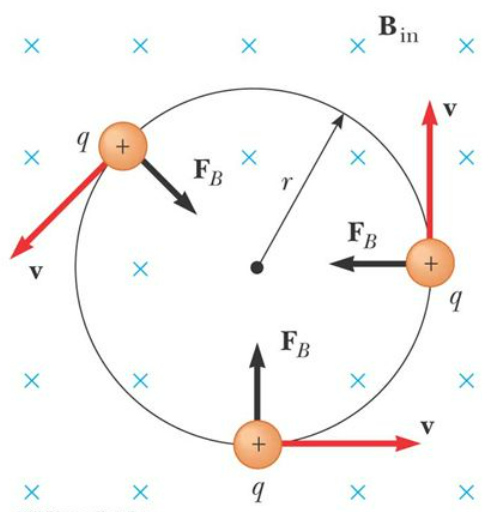
\includegraphics[width=8cm]{images/b_field_circularmotion.png}
\end{figure}

Period of revolution:
\[ T=\frac{2\pi r}{v} = \frac{2\pi\brac{\frac{mv}{Bq}}}{v} = \frac{2\pi m}{Bq} \] which is independent of $v$.

If $v$ and $B$ are not perpendicular, $0\degree < \theta < 90\degree$, charge moves in a helical path (i.e. it spirals forward).


\pagebreak

\subsubsection{Use of Crossed Fields}
Uniform $E$ and $B$ fields could be set up \underline{perpendicular} to each other such that they exert equal forces of opposite directions on a moving charged particle. This setup may be referred to as crossed fields.

A \textbf{velocity selector} emits a stream of charged particles (e.g. electrons) of a specific velocity.

\begin{figure}[H]
    \centering
    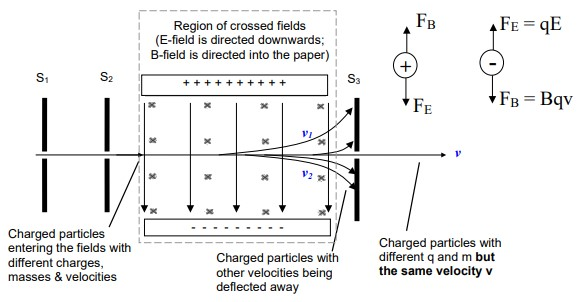
\includegraphics[width=14cm]{images/cross_fields.jpg}
\end{figure}

A beam of charged particles with a range of velocities $v_1,v_2,\dots,v_n$ pass through a region where there is a crossed field.

If the charged particles were electrons, then each electron in the crossed field experiences an upward electric force, and a downward magnetic force. (For positively charged particles: a downward electric force and an upward magnetic force)

For the particles to pass through undeflected, electric force and magnetic force are equal in magnitude:
\[ F_B = F_E \implies Bqv = qE \implies \boxed{v=\frac{E}{B}} \]
\pagebreak

\subsection*{Problems}


\pagebreak